\section{How often the proxy fails}
\label{sec:results}

We report separability first, because it does not depend on a chosen threshold, then the
false-hit/coverage trade-off (\cref{fig:frontier}), the score distributions that explain it,
and the operating points a deployment would actually run.

\begin{figure}[t]
  \centering
  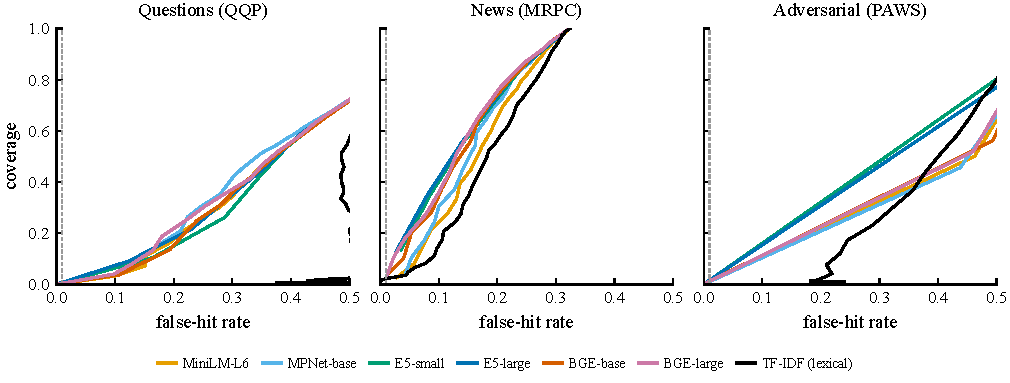
\includegraphics[width=\linewidth]{figures/fig_frontier}
  \caption{The cost of safety. Each curve sweeps the similarity threshold for one encoder;
    the vertical axis is coverage (the fraction of queries served) and the horizontal axis
    is the false-hit rate among those served. Up-and-to-the-left is better. The dashed line
    marks a $1\%$ false-hit ceiling. On questions and news, low-error operation costs most
    of the coverage; on the adversarial domain (right) the frontier collapses toward the
    diagonal, where coverage can be bought only by accepting an almost equal rate of wrong
    answers. Bands are $95\%$ bootstrap intervals.}
  \label{fig:frontier}
\end{figure}

\subsection{Separability across models and domains}
\label{sec:results-auc}
\Cref{fig:heatmap} and \cref{tab:separability} summarize threshold-free separability as
\prauc{} for every encoder--domain pair. Three patterns hold. First, the domain matters
more than the model. For a fixed encoder the spread of \prauc{} across domains is wide,
$0.62$ to $0.90$ for E5-large, while the spread across the six neural encoders within a
fixed domain is narrow, $0.54$ to $0.62$ on the adversarial set. Second, the adversarial
domain is close to unsolved: the best encoder reaches \prauc${}=0.62$ on \mbox{PAWS} against
a base rate of $0.44$, and its \rocauc{} of $0.67$ is barely above the $0.5$ of chance.
Scale buys little: moving from E5-small to E5-large raises \mbox{PAWS} \prauc{} by $0.08$,
and the \mbox{BGE} base-to-large gain is $0.04$. Third, and most telling, the lexical control
inverts the order. \mbox{TF-IDF} trails the neural encoders badly on questions, $0.49$
against $0.74$ to $0.78$, yet on the adversarial domain it \emph{outscores every neural
encoder}, $0.66$ against at most $0.62$. Word-scrambling defeats the semantics the neural
models encode, while the bigram structure the lexical model reads survives it. The very
property that makes an embedding useful, insensitivity to surface form, is what makes it
blind to an adversarial paraphrase.

\begin{figure}[t]
  \centering
  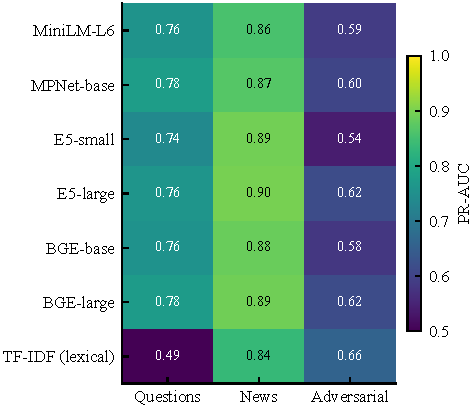
\includegraphics[width=0.82\linewidth]{figures/fig_heatmap}
  \caption{Threshold-free separability (\prauc{}) for each encoder and domain. Higher is
    better; the base rate of equivalent pairs is $0.36$ (questions), $0.68$ (news), and
    $0.44$ (adversarial). The adversarial column stays near the floor for every encoder.}
  \label{fig:heatmap}
\end{figure}

% Generated from results/reliability_summary.csv by experiments/make_tables.py
% Placeholder; regenerated by experiments/make_tables.py from results/reliability_summary.csv.
\begin{table}[t]
  \centering
  \begin{threeparttable}
    \caption{Threshold-free separability (\prauc{}) with $95\%$ bootstrap intervals, for
      every encoder and domain (placeholder; regenerated from results).}
    \label{tab:separability}
    \begin{tabular}{l c c c}
      \toprule
      Encoder & Questions & News & Adversarial \\
      \midrule
      MiniLM-L6 & -- & -- & -- \\
      \bottomrule
    \end{tabular}
  \end{threeparttable}
\end{table}


\subsection{The false-hit/coverage frontier}
\label{sec:results-frontier}
\Cref{fig:frontier} reads the same data as an operating curve. To hold the false-hit rate
under $1\%$, a deployment must move far up the threshold, and coverage falls with it. On
news the best encoder (E5-large) serves about $9\%$ of traffic at a $1\%$ ceiling; on
questions it serves under $1\%$; on the adversarial domain it serves essentially nothing.
Loosening the ceiling to $5\%$ raises news coverage to about $24\%$ but leaves questions
under $3\%$ and the adversarial domain under $1\%$. The news frontier is the most forgiving
because its pairs are the least lexically confusable; the adversarial frontier is the
warning, because it is the case a real cache meets whenever two prompts differ in a small
but decisive word.

\subsection{Why: the grey zone}
\label{sec:results-greyzone}
\Cref{fig:scores} shows where the failure comes from. For \mbox{BGE-large}, the similarity
scores of equivalent and non-equivalent pairs are well separated on questions but pile into
the same narrow, high band on the adversarial domain. On \mbox{PAWS} the median similarity
of equivalent and non-equivalent pairs differs by only $0.011$, both above $0.97$, against a
gap of $0.19$ on questions; no threshold can divide distributions that overlap this tightly.
A cache cannot act on a distinction its encoder does not represent, and on adversarial
near-duplicates the encoder does not represent it.

\begin{figure}[t]
  \centering
  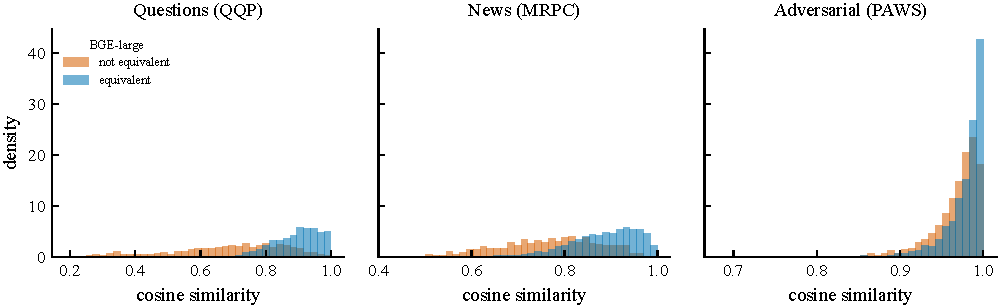
\includegraphics[width=\linewidth]{figures/fig_score_overlap}
  \caption{Similarity-score distributions for equivalent (blue) and non-equivalent (orange)
    pairs, for the strongest encoder, across the three domains. Separation on questions
    becomes near-total overlap on the adversarial domain, where both classes concentrate
    above $0.96$.}
  \label{fig:scores}
\end{figure}

\subsection{Operating points}
\label{sec:results-operating}
\Cref{fig:coverage} states the headline as a single number per encoder and domain: the
coverage a cache can deliver while keeping its false-hit rate at or below $1\%$. Across
encoders the achievable coverage is under $1\%$ on questions, between roughly $0.5\%$ and
$9\%$ on news, and below $0.5\%$ on the adversarial domain. The practitioner's takeaway is
blunt: a single global threshold chosen for a clean domain will leak false hits in a harder
one, and there is no threshold that makes the adversarial domain both safe and useful.

\begin{figure}[t]
  \centering
  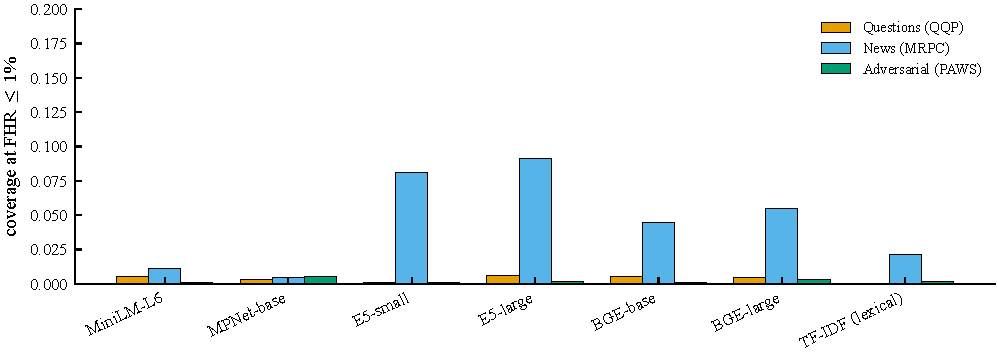
\includegraphics[width=\linewidth]{figures/fig_coverage_bars}
  \caption{Coverage achievable at a $1\%$ false-hit ceiling, per encoder and domain. Bars
    are $95\%$ bootstrap intervals. Even the strongest encoder serves only a small share of
    questions and news under the ceiling, and almost nothing on the adversarial domain.}
  \label{fig:coverage}
\end{figure}
